\documentclass[20pt, a1paper, portrait]{tikzposter}
\usepackage[utf8]{inputenc}
\usepackage{graphicx}
\usepackage{amsmath}

\graphicspath{{./images/}}



% RAJOUTER TITRE DU PROJET, AUTEURS
% 30% TEXTE, 40% ILLU, 30% VIDE
% PRECISER CHALLENGE TECHNIQUES
% RESULTATS
% CONCLUSION
% AMELIORATIONS, REFERENCES


\definebackgroundstyle{eurecom}{
\node[inner sep=0pt] at (0,0){
    
\includegraphics[width = \paperwidth,
    height = \paperheight]
    {poster-template.pdf}};
}

\usebackgroundstyle{eurecom}

\title{Visuwalk}
\titlegraphic{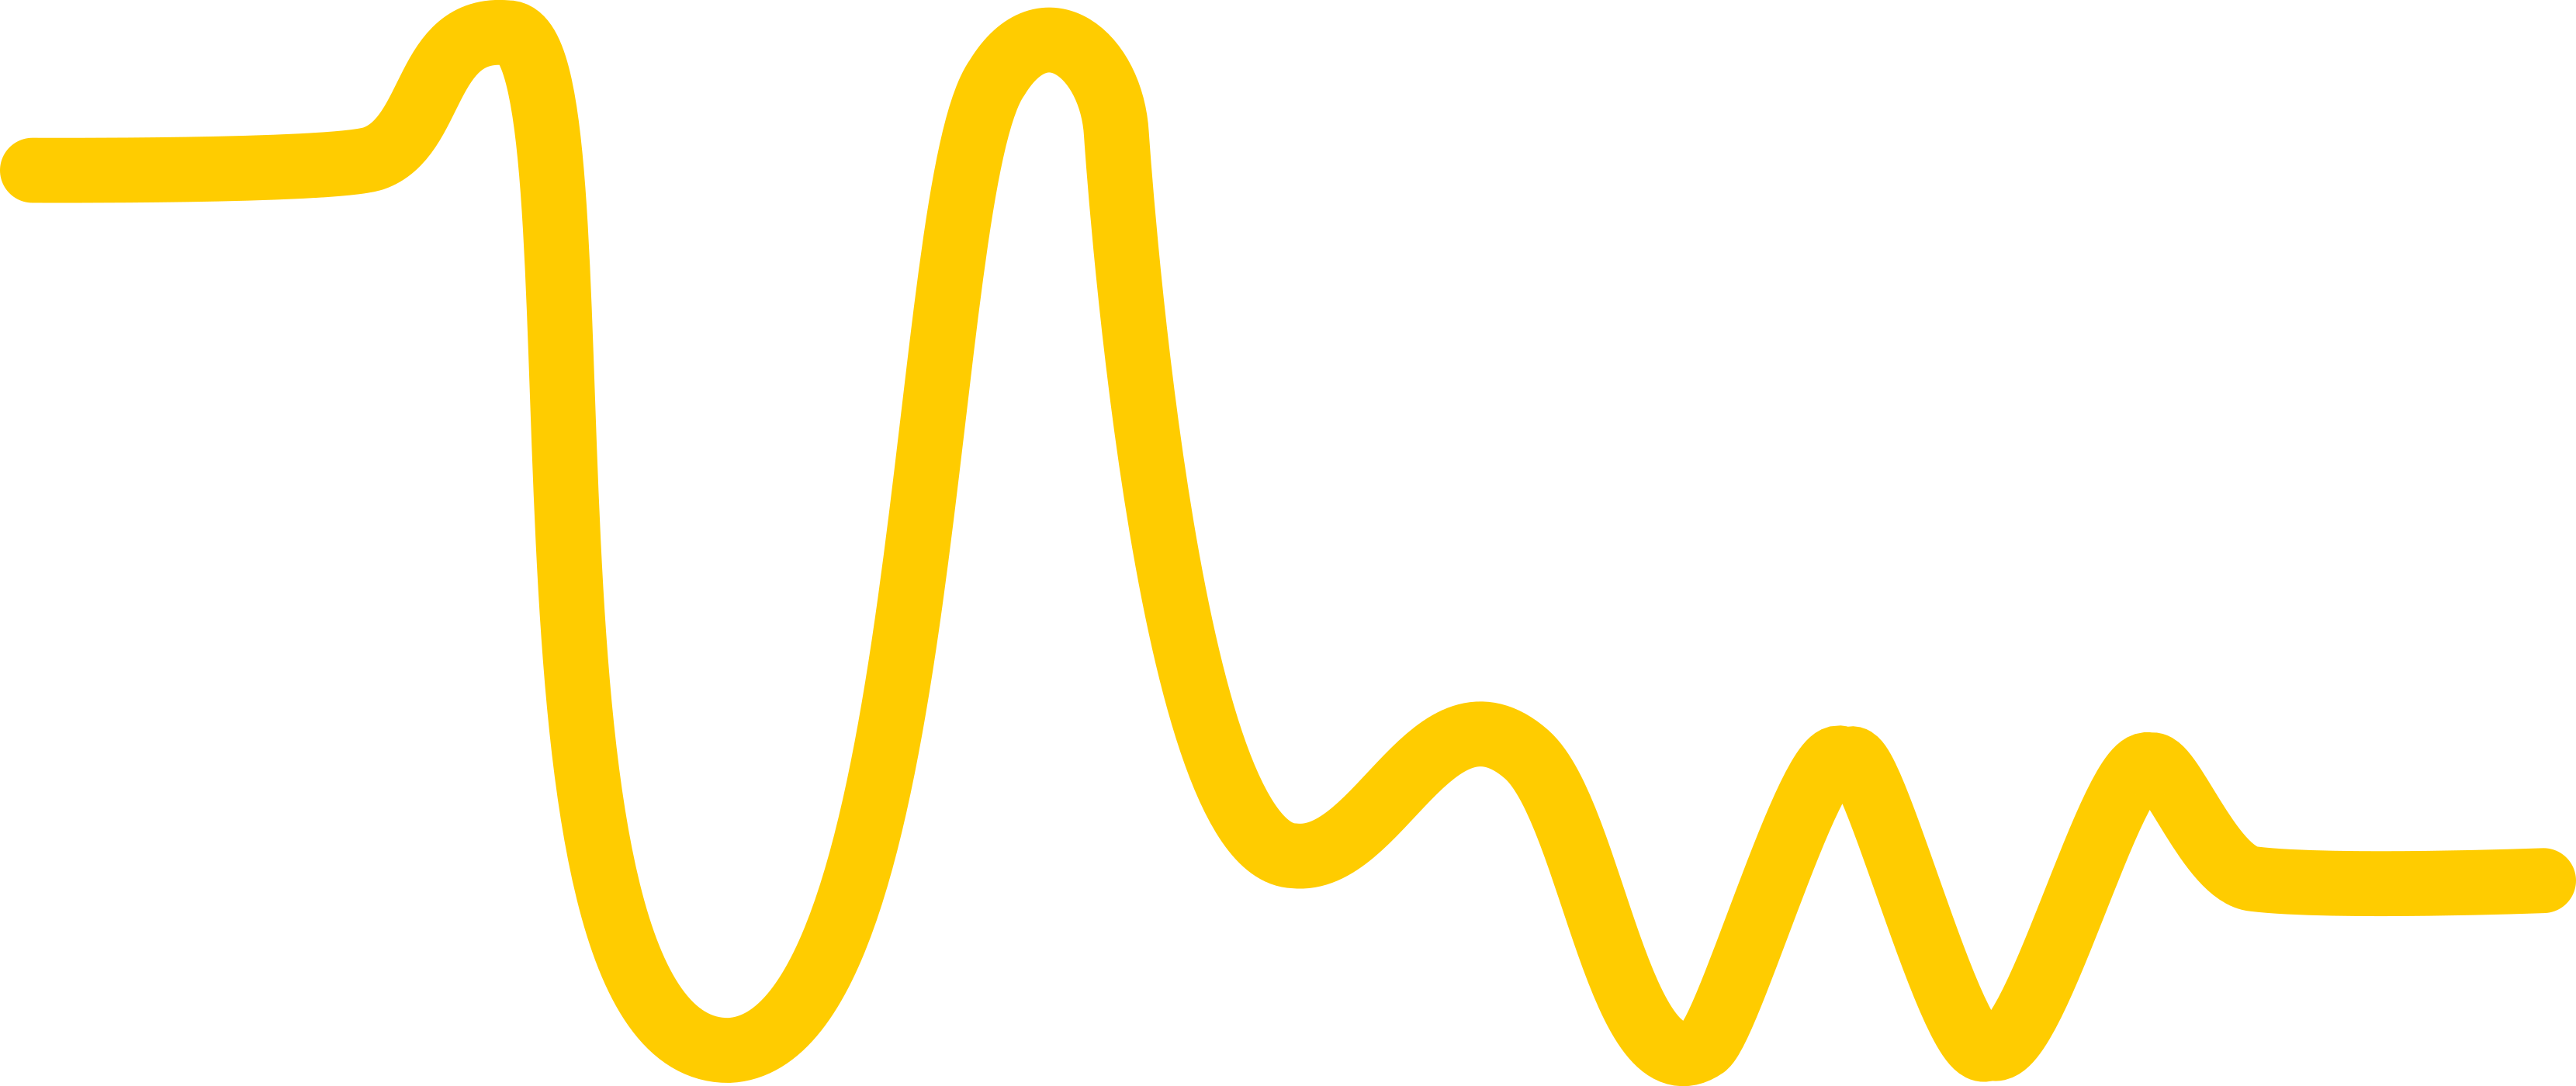
\includegraphics[width=0.15\paperwidth]{logo1.png}}
\author{\large Alexandre Avy, Hichem Khettab, Lou Marze, Hamza Parnica, Guillaume Ung}
\date{Semester 5}

\begin{document}

\maketitle

\block{\textbf{Abstract}}{

Medical aid for visually impaired people are numerous and come in various types, from a simple white cane to wearable haptic bracelets.
The goal of this project is to develop one of these medical aid, with the  following goal :
a visually impaired person must be able follow a curved line on the ground.
Using a Raspberry Pi 4 and its camera module, one has to : \\
- Process the video containing the line \\
- Send audio feedback to the user, guiding his walk \\
}

\begin{columns}

\column{0.5}

\block{
\textbf{Video / Image Processing}}{}

\block{
\textbf {Line detection}}{

In order to detect a line, multiple methods are available, such as convolution or the Hough transform for instance. Here, we decided to use the latter as it can directly detect any lines in any direction whereas convolution requires a different matrix for each direction. \\
Prior to applying a Hough transform, the image was converted to gray and applied a Canny edge detector to simplify this Hough transform. \\

Original image / Gray image / Canny edge + Hough transform image
}

\column{0.5}

\block{
\textbf {Guiding the user}}{
The first consideration we have to make before letting the user walk is to answer the following question : are the user’s feet on the line ?
Simply because if not, he will receive wrong instructions. \\


To resolve this, we decided to cut the frame in half (horizontally) and process these half frames separately.


Indeed, the bottom frame gives us information about the position of the user’s feet and thus, if the line is not in the center of the frame, then the user is not standing on the line.


To determine this, we just have to calculate the distance between the detected lines and the middle of the frame and if the distance is too high, then the user must move left or right. \\

Regarding the upper frame, it gives information about where the user should be heading next. To determine this, we decided to use the middle of the frame again but now by calculating the angle between the detected line and the middle vertical line. This way, we can tell how sharp of a turn the user has to make and whether it is left or right.
}

\block{}{
We choose \(\tau\) so that \(d_{95\%} = \frac{w}{2}\), thus we have
\[ 3\tau = \frac{w}{2}, \quad \tau = \frac{w}{6} \]
It follows,
\[f(d) = 1 - e^{\frac{-6d}{w}}\]
}

\block{\textbf{Sound Processing}}{}

\end{columns}

\end{document}
